% !TEX TS-program = XeLaTeX
% use the following command:
% all document files must be coded in UTF-8
\documentclass[portuguese]{textolivre}
% build HTML with: make4ht -e build.lua -c textolivre.cfg -x -u article "fn-in,svg,pic-align"

\journalname{Texto Livre}
\thevolume{19}
%\thenumber{1} % old template
\theyear{2026}
\receiveddate{\DTMdisplaydate{2025}{7}{6}{-1}} % YYYY MM DD
\accepteddate{\DTMdisplaydate{2025}{9}{5}{-1}}
\publisheddate{\DTMdisplaydate{2025}{11}{4}{-1}}
\corrauthor{Douglas Marin}
\articledoi{10.1590/1983-3652.2026.60147}
%\articleid{NNNN} % if the article ID is not the last 5 numbers of its DOI, provide it using \articleid{} commmand 
% list of available sesscions in the journal: articles, dossier, reports, essays, reviews, interviews, editorial
\articlesessionname{articles}
\runningauthor{Menezes, Costa e Marin} 
%\editorname{Leonardo Araújo} % old template
\sectioneditorname{Fernando Barbosa}
\layouteditorname{Saula Cecília}

\title{Análise a partir das Coreografias Didáticas da integração de tecnologias digitais no curso de licenciatura em Matemática}
\othertitle{Analysis based on the Didactic Choreographies of the integration of digital technologies in the bachelor’s degree in Mathematics}
% if there is a third language title, add here:
%\othertitle{Artikelvorlage zur Einreichung beim Texto Livre Journal}

\author[1]{Douglas Carvalho de Menezes~\orcid{0000-0003-0810-0500}\thanks{Email: \href{mailto:douglasmatufu@gmail.com}{douglasmatufu@gmail.com}}}
\author[2]{Muriell Francisco da Costa~\orcid{0000-0003-3019-3977}\thanks{Email: \href{mailto:muriell.francisco@ufu.br}{muriell.francisco@ufu.br}}}
\author[3]{Douglas Marin~\orcid{0000-0002-5798-5176}\thanks{Email: 
\href{mailto:douglasmarin@ufu.br}{douglasmarin@ufu.br}}}
\affil[1]{Escola Estadual João Pinheiro, Ituiutaba, MG, Brasil.}
\affil[2]{Colégio de Aplicação, Escola de Educação Básica, Uberlândia, MG, Brasil.}
\affil[3]{Universidade Federal de Uberlândia, Uberlândia, MG, Brasil.}

\addbibresource{article.bib}
% use biber instead of bibtex
% $ biber article

% used to create dummy text for the template file
\definecolor{dark-gray}{gray}{0.35} % color used to display dummy texts
\usepackage{lipsum}
\SetLipsumParListSurrounders{\colorlet{oldcolor}{.}\color{dark-gray}}{\color{oldcolor}}

% used here only to provide the XeLaTeX and BibTeX logos
\usepackage{hologo}

% if you use multirows in a table, include the multirow package
\usepackage{multirow}

% provides sidewaysfigure environment
\usepackage{rotating}

% CUSTOM EPIGRAPH - BEGIN 
%%% https://tex.stackexchange.com/questions/193178/specific-epigraph-style
\usepackage{epigraph}
\renewcommand\textflush{flushright}
\makeatletter
\newlength\epitextskip
\pretocmd{\@epitext}{\em}{}{}
\apptocmd{\@epitext}{\em}{}{}
\patchcmd{\epigraph}{\@epitext{#1}\\}{\@epitext{#1}\\[\epitextskip]}{}{}
\makeatother
\setlength\epigraphrule{0pt}
\setlength\epitextskip{0.5ex}
\setlength\epigraphwidth{.7\textwidth}
% CUSTOM EPIGRAPH - END

% to use IPA symbols in unicode add
%\usepackage{fontspec}
%\newfontfamily\ipafont{CMU Serif}
%\newcommand{\ipa}[1]{{\ipafont #1}}
% and in the text you may use the \ipa{...} command passing the symbols in unicode

% LANGUAGE - BEGIN
% ARABIC
% for languages that use special fonts, you must provide the typeface that will be used
% \setotherlanguage{arabic}
% \newfontfamily\arabicfont[Script=Arabic]{Amiri}
% \newfontfamily\arabicfontsf[Script=Arabic]{Amiri}
% \newfontfamily\arabicfonttt[Script=Arabic]{Amiri}
%
% in the article, to add arabic text use: \textlang{arabic}{ ... }
%
% RUSSIAN
% for russian text we also need to define fonts with support for Cyrillic script
% \usepackage{fontspec}
% \setotherlanguage{russian}
% \newfontfamily\cyrillicfont{Times New Roman}
% \newfontfamily\cyrillicfontsf{Times New Roman}[Script=Cyrillic]
% \newfontfamily\cyrillicfonttt{Times New Roman}[Script=Cyrillic]
%
% in the text use \begin{russian} ... \end{russian}
% LANGUAGE - END

% EMOJIS - BEGIN
% to use emoticons in your manuscript
% https://stackoverflow.com/questions/190145/how-to-insert-emoticons-in-latex/57076064
% using font Symbola, which has full support
% the font may be downloaded at:
% https://dn-works.com/ufas/
% add to preamble:
% \newfontfamily\Symbola{Symbola}
% in the text use:
% {\Symbola }
% EMOJIS - END

% LABEL REFERENCE TO DESCRIPTIVE LIST - BEGIN
% reference itens in a descriptive list using their labels instead of numbers
% insert the code below in the preambule:
%\makeatletter
%\let\orgdescriptionlabel\descriptionlabel
%\renewcommand*{\descriptionlabel}[1]{%
%  \let\orglabel\label
%  \let\label\@gobble
%  \phantomsection
%  \edef\@currentlabel{#1\unskip}%
%  \let\label\orglabel
%  \orgdescriptionlabel{#1}%
%}
%\makeatother
%
% in your document, use as illustraded here:
%\begin{description}
%  \item[first\label{itm1}] this is only an example;
%  % ...  add more items
%\end{description}
% LABEL REFERENCE TO DESCRIPTIVE LIST - END


% add line numbers for submission
%\usepackage{lineno}
%\linenumbers

\begin{document}
\maketitle

\begin{polyabstract}
\begin{abstract}
Neste texto, apresentam-se os resultados de um estudo realizado por meio de uma pesquisa qualitativa do tipo estudo de caso, cujo objetivo foi analisar como se proporcionou o desenvolvimento de uma disciplina para estudantes do ensino superior, os quais foram convidados a organizar uma proposta didática que dialogasse com Tecnologias Digitais de Informação e Comunicação (TDICs) para o ensino de Matemática, em uma universidade pública de Minas Gerais. Para atingir esse objetivo, foram utilizados os pressupostos metodológicos das Coreografias Didáticas, constituindo quatro eixos de análise, possibilitando compreender todo o cenário da pesquisa, a saber: a antecipação do aprendizado, a organização da disciplina, os aprendizados e os produtos. O estudo reforça a importância de disciplinas que integrem as TDICs nos cursos de licenciatura em Matemática, visando preparar futuros professores para um cenário educacional desafiador. Os resultados dessa pesquisa demonstraram que, quando bem aplicadas, as TDICs podem ser aliadas eficazes no ensino e na aprendizagem, contribuindo para a formação docente. Por fim, recomenda-se que estudos futuros analisem os impactos de longo prazo dessas formações na prática dos licenciandos e explorem novas metodologias e ferramentas tecnológicas para melhorar o ensino de Matemática na Educação Básica.

\keywords{Tecnologias Digitais de Informação e Comunicação\sep Formação docente\sep Coreografias Didáticas}
\end{abstract}

\begin{english}
\begin{abstract}
This text presents the results of a qualitative case study, the aim of which was to analyze how a subject was developed for higher education students, who were invited to organize a didactic proposal that dialogued with Digital Information and Communication Technologies (DICTs) for teaching mathematics at a public university in Minas Gerais. To achieve this goal, the methodological assumptions of Didactic Choreographies were used, constituting four axes of analysis, making it possible to understand the entire research scenario, namely: the anticipation of learning, the organization of the discipline, the learning and the products. The study reinforces the importance of subjects that integrate DICTs in mathematics degree courses, with the aim of preparing future teachers for a challenging educational scenario. The results of this research have shown that, when properly applied, DICTs can be effective allies in teaching and learning, contributing to teacher training. Finally, it is recommended that future studies analyze the long-term impact of this training on the practice of undergraduates and explore new methodologies and technological tools to improve the teaching of mathematics in Basic Education.

\keywords{Digital Information and Communication Technologies\sep Teacher training\sep Didactic Choreographies}
\end{abstract}
\end{english}
% if there is another abstract, insert it here using the same scheme
\end{polyabstract}

\section{Introdução}\label{sec-intro}
As Tecnologias Digitais de Informação e Comunicação (TDICs) estão cada vez mais presentes na vida das pessoas, em diferentes setores da sociedade, permeando cotidianos e criando diversas culturas. Uma dessas culturas presentes na sociedade é a cultura digital que modela as formas de pensar, agir e comunicar-se no convívio social. Essa realidade permite originar novas dinâmicas de interação e esses novos comportamentos redefinem as relações com o mundo.

Esses movimentos têm influenciado na transformação dos hábitos das pessoas, que diariamente realizam suas atividades por meio de recursos tecnológicos ou meios de comunicação de fácil acesso à \textit{internet} a qual proporciona uma fonte inesgotável de informações.

No que compete ao ensino ``[…] usamos muitos tipos de tecnologias para aprender e saber mais e precisamos da educação para aprender e saber mais sobre as tecnologias'' \cite[p. 44]{kenski2007}. Por outro lado, o processo de incorporação do uso das TDICs, em especial, para estudos, aquisição de novos saberes, bem como para o desenvolvimento de novas habilidades cognitivas, ``sua integração em atividades curriculares demandam tempo e acontecem de modo gradativo'' \cite[p. 44]{almeida2011}.

A Base Nacional Comum Curricular (BNCC) corrobora com essas reflexões e aponta para a necessidade de:

\begin{quote}
    compreender, utilizar e criar tecnologias digitais de informação e comunicação de forma crítica, significativa, reflexiva e ética nas diversas práticas sociais (incluindo as escolares) para se comunicar, acessar e disseminar informações, produzir conhecimentos, resolver problemas e exercer protagonismo e autoria na vida pessoal e coletiva \cite[p. 9]{brasil2018}.
\end{quote}

De tal forma, para fomentar essas propostas, percebemos que o professor precisa estar disposto a lidar com a diversidade e a abrangência que demandam ao utilizar as TDICs para o ensino. Nesse sentido, \textcite[p. 144]{valente2014} enfatiza a necessidade do docente de compreender como proporcionar a conversão de informação em conhecimento pelo usuário, argumentando que o ``[…] processo educacional é saber como prover as informações, de modo que ela possa ser interpretada pelo aprendiz que passa a entender quais ações ele deve realizar para que a informação seja convertida em conhecimento''.

Sendo assim, os cursos de formação inicial de professores para a Educação Básica precisam estruturar seus currículos de modo a assegurar

\begin{quote}
    […] a presença de sólida formação que propicie o conhecimento dos fundamentos epistemológicos, técnicos e ético-políticos das ciências da educação e da aprendizagem e que permita ao futuro profissional do magistério o desenvolvimento das capacidades de análise e reflexão sobre as práticas educativas e sobre a progressão e os processos de aprendizagem e o aprimoramento constante de suas competências de trabalho \cite[p. 3]{brasil2024}.
\end{quote}

No cenário dos cursos de licenciatura em Matemática,

\begin{quote}
    […] ao chegar à Universidade, o aluno já passou por um longo processo de aprendizagem escolar e construiu para si uma imagem dos conceitos matemáticos a que foi exposto, durante o ensino básico. Assim, a formação do matemático demanda o aprofundamento da compreensão dos significados dos conceitos matemáticos, a fim de que ele possa contextualizá-los adequadamente \cite[p. 4]{brasil2001}.
\end{quote}

É nesse contexto que este texto pretende contribuir, ao analisar como se proporcionou o desenvolvimento de uma disciplina para estudantes do ensino superior, os quais foram convidados a organizar uma proposta didática que dialogasse com o TDIC para o ensino de Matemática.

Para atingir esse objetivo, nos apoiaremos nos conceitos das Coreografias Didáticas, discutidas por \textcite{oser2001, padilha2016, costa2023}. Esse direcionamento teórico vai além da orientação e explicação dos elementos curriculares, sendo organizados em quatro níveis, a saber: a antecipação, a colocação em cena, os aprendizados e o produto.


\section{Contexto}
Este estudo teve como cenário o curso de graduação em licenciatura em Matemática, ofertado pelo Instituto de Matemática e Estatística (IME), da Universidade Federal de Uberlândia (UFU), no estado de Minas Gerais.

O curso possui carga horária de 3030 horas de conteúdos específicos e pedagógicos, sendo 405 horas dedicadas à prática como componente curricular e 405 horas para o estágio supervisionado. Ademais, 200 horas são destinadas para atividades científico-culturais, totalizando 3230 horas de integralização a ser cumprida pelo discente em Matemática. Essa carga horária é distribuída em 39 disciplinas, organizadas em oito períodos letivos, ofertado de modo semestral \cite{instituto2018}.

A pesquisa foi realizada no componente curricular Informática e Ensino, que possui uma carga horária de 90 horas, sendo oferecida ao terceiro período do curso. Esse componente curricular apresenta em sua ementa, o objetivo de ``implementar práticas educativas com tecnologias digitais da informação e comunicação no processo de ensinar e aprender matemática'' \cite[p. 72]{instituto2018}.

Além disso, essa disciplina está inserida ao Projeto Interdisciplinar (Prointer), que segundo o Projeto Institucional da UFU, possui caráter obrigatório a todos os cursos de licenciatura da instituição e tem como propósito o de:

\begin{quote}
I -- promover a articulação teoria-prática durante toda formação do estudante; \\
II -- articular e aprofundar temáticas que consolidem os objetivos da formação de professor nas diversas áreas que compõem a estrutura curricular;\\
III -- compreender a escola e os espaços não escolares como propícios à reflexão teórico-prática;\\
IV -- inserir o licenciando na realidade concreta das instituições escolares e não escolares - sensibilização, observação, diagnóstico, problematização, elaboração de propostas que atendam à realidade do contexto observado, com o fortalecimento da identidade docente; \\
V -- possibilitar que o estudante seja capaz de refazer o processo de pesquisa e discutir metodologias e resultados, tendo em vista ampliar a compreensão a respeito dos contextos educacionais e de seus condicionantes e desenvolver o espírito investigativo, por meio de pesquisas que problematizem o cotidiano escolar; \\
VI -- problematizar o contexto educacional em que os projetos serão desenvolvidos e, a partir disso, construir alternativas para solucionar os problemas detectados, numa perspectiva colaborativa com as escolas e demais espaços educativos; e \\
VII -- possibilitar análise sociopolítica, administrativa e pedagógica da realidade como ação inicial para aprofundamento no estágio, este caracterizado pela imersão/mergulho na complexidade das instituições escolares e não escolares \cite[p. 7]{universidade2017}.
\end{quote}

À vista disso, entende-se que esse componente curricular se caracteriza como um espaço para discussões ligadas à formação profissional, voltadas para compreensão de práticas educacionais distintas e de diferentes aspectos da cultura das instituições de Educação Básica. Outrossim, no Projeto Político Pedagógico do curso, esse componente curricular comparece a implementação de propostas educativas que envolvam as TDICs para o ensino de Matemática no contexto escolar \cite{instituto2018}.

As orientações educacionais presentes na BNCC acerca do uso das TDICs preconizam o itinerário que o futuro professor de Matemática precisa desenvolver acerca da capacidade de utilizar as tecnologias digitais de forma crítica e criativa, elaborando propostas didáticas que problematizam conceitos matemáticos e situações do cotidiano em contextos de ensino. Para que esse objetivo seja alcançado, a formação inicial em Matemática deve assegurar ao estudante não apenas o domínio dos conteúdos específicos da área, mas também o desenvolvimento de um conjunto de habilidades e competências essenciais ao longo do percurso formativo, tais como a articulação entre teoria e prática, a reflexão crítica sobre os processos de ensino e aprendizagem e a mobilização de recursos didático-pedagógicos adequados às diferentes realidades escolares.

\begin{quote}
Desde o início do curso e licenciando deve adquirir familiaridade com o uso do computador como instrumento de trabalho, incentivando-se sua utilização para o ensino de matemática, em especial para a formulação e solução de problemas. É importante também a familiarização do licenciando, ao longo do curso, com outras tecnologias que possam contribuir para o ensino de Matemática \cite[p. 6]{brasil2001}.
\end{quote}

A partir desse enredo, propõe-se analisar como se proporcionou o desenvolvimento de uma disciplina para estudantes do ensino superior, os quais foram convidados a organizar uma proposta didática que dialogasse com o TDIC para o ensino de Matemática. Sendo assim, apresenta-se o modo em que foi organizado esse componente curricular, assim como a fundamentação teórica que o sustenta para atingir o objetivo deste texto.

\section{Coreografias Didáticas}
No campo das ciências educacionais, inúmeras discussões giram em torno da formação de professores e de como esses estudos se relacionam com estratégias para promover novas abordagens didáticas. A busca pela inovação é constante nesse contexto, impulsionada pelas complexidades presentes rotineiramente nos ambientes educacionais. Isso estimula a adoção de múltiplas abordagens metodológicas, visto a necessidade de promover o aprendizado de forma criativa e inovadora.

Nesse contexto, surgem modelos que visam auxiliar na inovação da prática docente, intrinsecamente associados a elementos que visam aprimorar as abordagens tradicionais mais utilizadas pelos professores, como os paradigmas das aulas expositivas, a reprodução do conhecimento, a atividades de cópia e repetição, bem como a abordagem hierárquica na transmissão e memorização do conhecimento. Todavia, o processo educativo com o(s) modelo(s) didático(s) torna-se um elemento que auxilia a (re)pensar como novas abordagens de ensino podem ser elaboradas, visto a necessidade de alcançar os objetivos do currículo para a aprendizagem \cite{costa2023}.

Sendo assim, considera-se relevante pensar como modelos didáticos influenciam os processos cognitivos, tornando o conhecimento mais envolvente seja qual for o público-alvo. Desse modo, com o objetivo de auxiliar na melhoria das abordagens docentes ao buscar promover o ensino, \textcite{oser2001} conduziram um estudo sobre as Coreografias Didáticas. Esse modelo didático para o ensino propõe ações que visam aprimorar o processo educacional. Os professores são incentivados a criar ``coreografias de ensino'', ou seja, estratégias que promovam a reflexão sobre os modelos-base de aprendizagem \cite{padilha2016, costa2023}. Essas coreografias envolvem movimentos cuidadosamente planejados, como a seleção de recursos, materiais e ferramentas educacionais, a organização das atividades em sala de aula e a adaptação do ensino ao perfil dos(as) estudantes.

Dessa maneira, ao invés de seguir uma abordagem estática ou até mesmo seguindo a coreografia tradicional do ensino, as Coreografias Didáticas incentivam a flexibilidade e a criatividade, pois se ``serve[m] da arte de compor e aprimorar as capacidades de aprendizagem dos estudantes e o papel de ensinar atribuído ao professor(a)'' \cite[p. 79]{costa2023}. Um modelo didático de Coreografia Didática que incorpora esse cenário de integração das TDICs no ensino superior está pautado em ``[…] uma inovação nas práticas docentes que supera a abordagem tradicional, baseada num paradigma de reprodução de conhecimento'' \cite[p. 1]{padilha2016}.

Para os autores, ao inovar com a TDIC para o ensino superior por meio das Coreografias Didáticas, assegura-se:

\begin{quote}
[…] a promoção de práticas pedagógicas que favoreçam a flexibilização curricular, com foco na aprendizagem do aluno, na autonomia, no pensamento crítico e na reflexão sobre o seu próprio processo de aprendizagem e a indissociação entre ensino e aprendizagem, rompendo com um ensino tradicional, mecânico e memorístico, focado na ação do professor. A principal inovação que aconteceu nos últimos anos foi a transferência do centro de atenção do ensino para a aprendizagem. Esse fator permitiu, assim, uma reconfiguração geral em como compreendemos o ensino e o papel do professor no processo educativo \cite[p. 1]{padilha2016}.
\end{quote}

Dessa maneira, os professores podem ajustar suas estratégias conforme as necessidades dos alunos, tornando o processo de ensino mais dinâmico e atendendo às necessidades educacionais. Por conseguinte, o pressuposto metodológico das Coreografias Didáticas se estabelece primordialmente no planejamento da aula em que professores incorporam estratégias dinâmicas em suas práticas de ensino, de modo que:

\begin{quote}
    
os professores são coreógrafos dos contextos de aprendizagem dos seus alunos. Eles organizam coreografias (externas) que `postas em cena' modulam o processo de aprendizagem dos estudantes (coreografias internas) \cite{zabalza2006competencias}, na mobilização e produção de suas capacidades pessoais. Essas coreografias podem ocorrer tanto em situações de ensino presenciais como virtuais e os cenários em que ocorrem essas coreografias podem ir do mais minimalista possível ao mais elaborado, no que se refere a estratégias e recursos didático-tecnológicos \cite[p. 2-3]{padilha2016}.
\end{quote}

Em resumo, essa abordagem para o ensino busca não apenas transmitir informações, mas também criar um diálogo harmonioso entre o conhecimento, a reflexão e a prática em sala de aula \cite{costa2023}. Assim, na parte operacional de uma Coreografia Didática, ela é compreendida por quatro níveis de atuação e de articulação cíclica, a saber: a antecipação, a colocação em cena, os aprendizados (modelos-bases de aprendizagem) e o produto (Figura \ref{fig-1}).

%--- CÓDIGO DA FIGURA 1 ---%
\begin{figure}[h!]
\centering
\begin{minipage}{0.95\textwidth}
\includegraphics[width =\textwidth]{Imagens/image1.png}
\caption{Operacionalização das Coreografias Didáticas.}
\label{fig-1}
\source{Desenvolvido pelos autores (2025), adaptado de \textcite{costa2023}.}
\end{minipage}
\end{figure}

Ao considerar a proposta de operacionalização das Coreografias Didáticas conforme Figura \ref{fig-1}, entende-se que esses níveis de ações estão conectados e desafiam o paradigma da linearidade no processo de aprendizado, a saber, o tradicionalismo educacional, conhecida como a coreografia tradicional do ensino. Essa abordagem sugere uma convergência entre o planejamento do ensino e o desenvolvimento da aprendizagem, por meio das interações entre professores(as) e estudantes, tanto na estrutura visível quanto na invisível. Como afirmam \textcite{padilha2016}, essa abordagem torna mais nítida a interdependência e a articulação entre esses elementos.

A literatura científica sobre as Coreografias Didáticas promove uma visão dinâmica e integrada do processo educacional por meio desse pressuposto metodológico, como também ``refletem sobre como nem sempre a intenção de ensino atinge o real aprendizado dos alunos'' \cite[p. 51]{padilha2016}. Dessa maneira, essa abordagem propõe indicar novos caminhos para o professor compreender a forma como as operações mentais internas do estudante tendem a estabelecer conexões com o aprendizado que é proposto. Assim, ``o professor, ao definir suas atividades de ensino (estrutura visível da coreografia), deve ter em mente que ações cognitivas (estrutura invisível das coreografias) as atividades propostas vão provocar em seus alunos'' \cite[p. 9]{padilha2016}.

Deste modo, o pressuposto metodológico das Coreografias Didáticas se ocupou, neste texto, de encaminhar a construção dos eixos de análise de informações obtidas em campo, cujo intuito foi de sistematizar, apresentar e compreender conforme preconizado nos objetivos anteriormente.


\section{Metodologia}
Neste estudo foi utilizada uma pesquisa de natureza qualitativa tendo em vista que o interesse está em compreender como foi desenvolvida uma disciplina para estudantes do ensino superior, os quais foram convidados a organizar uma proposta didática que dialogue com as TDICs para o ensino de Matemática.

Tal interpretação está de acordo com \textcite[p. 47]{bogdan1994}, quando dizem que ``na investigação qualitativa a fonte direta de dados é o ambiente natural constituindo o investigador o instrumento principal''. Dessa forma, o pesquisador acompanha diretamente o cenário do estudo, em outras palavras, o ambiente natural é uma fonte direta para a produção dos dados apoiados nos participantes, valorizando as suas percepções, opiniões e relatos \cite{borba2020}.

Posto isso, utilizou-se o estudo de caso que ``não é uma técnica específica, mas uma análise holística, a mais completa possível, que considera a unidade social estudada como um todo'' \cite[p. 33]{goldenberg2007}. A autora indica que esse método reúne o maior número de informações detalhadas, com o objetivo de apreender a totalidade de uma situação e descrever a complexidade de um caso concreto.

Dando continuidade, a investigação foi desenvolvida na disciplina Informática e Ensino do curso de graduação em licenciatura em Matemática, ofertada no Instituto de Matemática e Estatística na Universidade Federal de Uberlândia (UFU). Os participantes foram oito estudantes, matriculados na componente curricular: Bianca, Davi, Elias, Gabriel, Kleber, Luís, Maitê e Paulo\footnote{Foram utilizados pseudônimos para preservar a identificação dos participantes na pesquisa. O Certificado de Apresentação de Apreciação Ética (CAAE) gerado pelo Comitê de Ética em Pesquisas (CEP/UFU) e que apresenta o parecer aprovado para a realização dessa pesquisa é: 68582523.4.0000.5152.}.

O estudo de campo ocorreu no acompanhamento da disciplina, que foi desenvolvida no período de 8 de janeiro de 2024 a 9 de maio 2024, compreendido como o segundo semestre de 2023\footnote{Devido à pandemia do COVID-19, o calendário acadêmico da universidade ainda não está atualizado até o momento da escrita deste artigo.}. Ao longo do semestre, os licenciandos discutiram artigos científicos, participaram de palestras e oficinas de conteúdo específicos de matemática básica com o uso do \textit{software} GeoGebra e assistiram vídeos, todas essas modalidades de estudo sempre envolvendo as TDICs. Após essas atividades, o grupo de participantes foi convidado a organizar uma proposta didática que dialogasse com as TDICs para o ensino de Matemática.

Os dados da pesquisa consistiram em registros escritos feitos pelo professor, notas de observação feitas no caderno de campo de um dos pesquisadores que esteve inserido no contexto da pesquisa participando efetivamente das aulas, formulários respondidos por meio do Google Forms e da entrega da proposta didática elaborada pelos licenciandos.

Para os eixos de análise, utilizaram-se os conceitos da Coreografias Didáticas discutidos em \textcite{oser2001}, \textcite{padilha2016} e \textcite{costa2023}, que, segundo esses autores, são organizados em quatro níveis: a antecipação do aprendizado, a colocação em cena, os aprendizados e o produto.

Esses quatros eixos de análise são apresentados a seguir, tendo a proposta de configurar uma compreensão holística e dinâmica do processo de ensino e aprendizagem, no qual as TDICs são integradas ao contexto formativo dos licenciandos(as). Através desses eixos, procurou-se compreender as diferentes fases do processo pedagógico, desde o planejamento até a materialização dos resultados, levando em conta as interações entre o professor da disciplina, os(as) estudantes e as tecnologias utilizadas.


\section{Discussões}
Com vistas a assegurar maior rigor metodológico e clareza expositiva, esta seção está organizada em quatro subseções, que correspondem às etapas constitutivas das Coreografias Didáticas \cite{oser2001, padilha2016, costa2023}. Em cada subseção, delineiam-se os procedimentos adotados, as ações desenvolvidas e os resultados parciais obtidos, de modo a evidenciar o percurso investigativo e a fundamentação analítica de cada fase do estudo realizado.


\subsection{A antecipação do aprendizado}
Para desenvolver as aprendizagens com os estudantes na disciplina, o docente do componente curricular aplicou um formulário do Google Forms para entender o nível de conhecimento dos discentes em relação aos tópicos que seriam abordados. Esses tópicos incluíam: Ambiente Virtual de Aprendizagem, \textit{softwares} nas aulas de Matemática e projetos de informática no ensino e aprendizagem de Matemática.

Dentre as perguntas do formulário, uma delas foi sobre o local de acesso à \textit{internet} dos estudantes. Conforme mostrado na \Cref{fig-graf-1}, todos os seis que responderam o formulário indicaram que tinham acesso tanto em casa quanto na universidade. Isso nos permite concluir que os discentes possuíam os recursos necessários para acessar plataformas de ensino, como Moodle, Google Classroom, entre outras.

%--- código do gráfico 1 ---%
\begin{figure}[h!]
\centering
\begin{minipage}{0.95\textwidth}
\includegraphics[width =\textwidth]{Imagens/grafico1.png}
\caption{Respostas dos estudantes sobre o local de acesso à \textit{internet}.}
\label{fig-graf-1}
\source{Desenvolvido pelos autores (2025).}
\end{minipage}
\end{figure}

Como o docente da disciplina Informática e Ensino planejava utilizar o Ambiente Virtual de Aprendizagem (AVA) Moodle, ele incluiu no formulário uma pergunta sobre quais AVAs os estudantes conheciam, conforme ilustrado na \Cref{fig-graf-2}.

%--- código do gráfico 2 ---%
\begin{figure}[h!]
\centering
\begin{minipage}{0.95\textwidth}
\includegraphics[width =\textwidth]{Imagens/grafico2.png}
\caption{Respostas dos estudantes sobre quais AVAs conheciam.}
\label{fig-graf-2}
\source{Desenvolvido pelos autores (2025).}
\end{minipage}
\end{figure}

Ao analisar as respostas dos estudantes, é possível observar que todos os seis que responderam o formulário tinham conhecimento do AVA Moodle e do Google Classroom. Portanto, o planejamento do professor poderia ser implementado, dado que os estudantes estavam familiarizados com esses dois Ambientes Virtuais de Aprendizagem. Outra pergunta feita aos discentes no formulário foi sobre como eles classificavam seu domínio sobre as TDICs para ensinar e aprender Matemática.

%--- código do gráfico 3 ---%
\begin{figure}[h!]
\centering
\begin{minipage}{0.75\textwidth}
\includegraphics[width =\textwidth]{Imagens/grafico3.png}
\caption{Respostas dos estudantes sobre como classificavam seu domínio das TDIC.}
\label{fig-graf-3}
\source{Desenvolvido pelos autores (2025).}
\end{minipage}
\end{figure}

Ao analisar a \Cref{fig-graf-3}, nota-se que três estudantes consideram ter um bom domínio na utilização das TDICs para ensinar e aprender Matemática. Dois discentes avaliam seu domínio como regular, enquanto um estudante acredita ter um conhecimento fraco em relação ao uso das TDICs para esses fins. Dessa forma, conclui-se que a disciplina é importante para o fortalecimento de aprendizados ao utilizar as TDICs no ensino e aprendizado da Matemática.

Posteriormente, os estudantes foram consultados por meio do formulário sobre suas recomendações para o uso das TDICs no ensino de Matemática.

%--- código do gráfico 4 ---%
\begin{figure}[h!]
\centering
\begin{minipage}{0.75\textwidth}
\includegraphics[width =\textwidth]{Imagens/grafico4.png}
\caption{Respostas dos estudantes sobre o uso das TDIC durante as aulas.}
\label{fig-graf-4}
\source{Desenvolvido pelos autores (2025).}
\end{minipage}
\end{figure}

Ao observar a \Cref{fig-graf-4}, percebe-se que os estudantes consideram importante o uso das TDICs durante as aulas de Matemática. Eles acreditam que o professor deve utilizar essas tecnologias para ensinar os conteúdos explorados em suas aulas. Para isso, o professor precisa estar familiarizado com esses recursos.

Para os estudantes, como Maitê, ``[…] deve-se saber como utilizar a fim de atingir os objetivos educacionais''. Luís acrescenta que a utilização das TDICs para o ensino e aprendizagem de Matemática ``[…] pode ser muito benéfica, desde que seja bem usada, visto que não basta apenas levar a tecnologia para a sala de aula, mas também saber onde colocá-la''.

Dessa forma, o planejamento da disciplina Informática e Ensino visava proporcionar aos estudantes a familiarização com os AVA Moodle e Google Classroom, além de outras TDICs, preparando-os para o uso efetivo dessas ferramentas no processo de ensino e aprendizagem. Conforme a estudante Maitê narra, ``[…] devido à presença forte da tecnologia em todas as áreas da vida, acredito que não há como fugir desse recurso para o ensino de Matemática''. Essa preparação é essencial para integrar as tecnologias de maneira eficaz e significativa no contexto educacional.


\subsection{A organização da disciplina}
O componente curricular de Informática e Ensino, também conhecida como Prointer II, possui uma carga horária prática de noventa horas. Ela pertence ao quadro de disciplinas obrigatórias do curso de graduação em licenciatura em Matemática e bacharelado em Matemática, sendo ofertada no terceiro período. Essa disciplina tem como objetivo ``implementar práticas educativas com tecnologias digitais da informação e comunicação no processo de ensinar e aprender matemática'' \cite[p. 72]{instituto2018}.

Por essa disciplina fazer parte do núcleo formativo do Prointer, o intuito é que seus conteúdos sejam desenvolvidos através de ações integradas com a participação contínua dos discentes. Com tal característica, pretende-se promover a articulação entre teoria e a prática na formação do estudante, articulando e aprofundando temáticas que consolidam os objetivos da formação de professor nas diversas áreas que compõem a estrutura curricular do curso de Matemática, possibilitando que o estudante seja capaz de refazer o processo de pesquisa, discutindo essa específica metodologia de ensino-aprendizagem, tendo em vista ampliar a compreensão a respeito dos contextos educacionais em um ambiente tecnológico \cite{instituto2018}.

O programa de conteúdo da disciplina está dividido em (1) Ambiente Virtual de Aprendizagem, (2) Objetos de Aprendizagem de Matemática, (3) Softwares nas aulas de Matemática e (4) Projetos de informática no ensino e aprendizagem de Matemática. Essa organização pode ser observada na Figura \ref{fig-2}.

%--- código da figura 2 ---%
\begin{figure}[h!]
\centering
\begin{minipage}{0.90\textwidth}
\includegraphics[width =\textwidth]{Imagens/image2.png}
\caption{Programa de conteúdos da disciplina.}
\label{fig-2}
\source{Desenvolvido pelos autores (2025), adaptado de \textcite{instituto2018}.}
\end{minipage}
\end{figure}

Com o avanço das TDICs, seu uso na Educação é perceptível nas diferentes instituições escolares espalhadas pelo país. Os recursos digitais são variados e incluem plataformas virtuais, jogos, aplicativos, sites da \textit{internet}, celulares, câmeras, \textit{tablets} e projetores. Todos esses recursos podem tornar o aprendizado de Matemática mais interessante e envolvente para os estudantes.

Nesse sentido, mobilizou-se o desenvolvimento e a confecção do Projeto Digital. A proposta desse recurso didático foi associar temas envolvendo tecnologias com a Matemática. Como o foco estava nos futuros professores de Matemática, objetivou-se utilizar temáticas voltadas para o ensino da Educação Básica, conforme ilustrado na Figura \ref{fig-3}.

%--- código da figura 3 ---%
\begin{figure}[h!]
\centering
\begin{minipage}{0.90\textwidth}
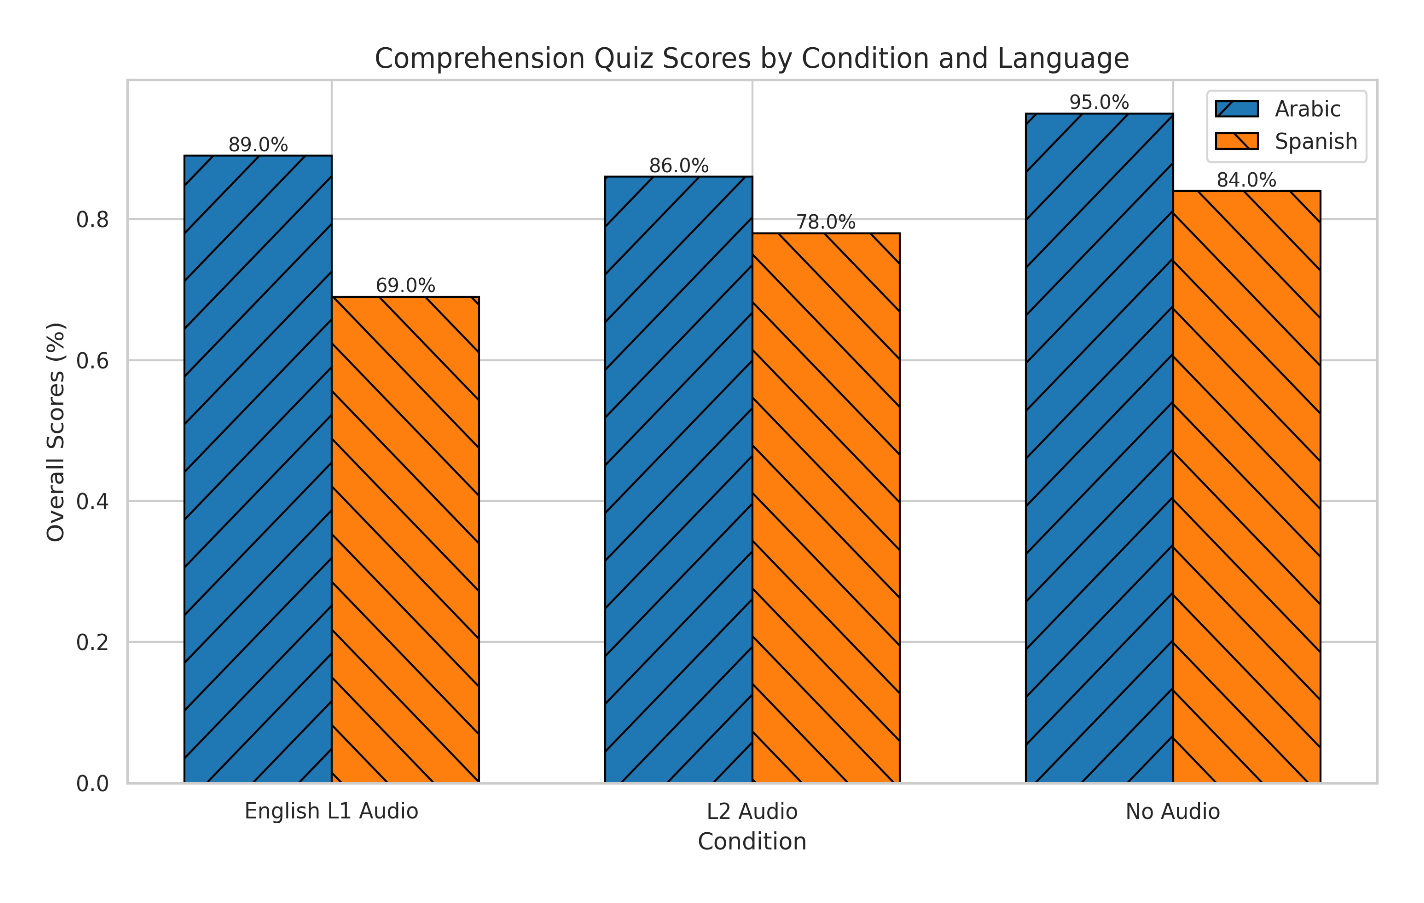
\includegraphics[width =\textwidth]{Imagens/image3.png}
\caption{Temas para serem desenvolvidos pelos estudantes.}
\label{fig-3}
\source{Desenvolvido pelos autores (2025).}
\end{minipage}
\end{figure}

Os estudantes da disciplina tiveram liberdade de escolher o tema e o conteúdo que mais lhes interessavam. Durante as discussões, houve o acréscimo da temática da Inteligência Artificial (IA), como as IAs generativas do ChatGPT, assim como a possibilidade da livre escolha, permitindo que os temas pudessem ser repetidos entre os participantes. Assim, ficou a distribuição entre os estudantes, conforme a \Cref{tab-quadro-1}.

%--- código do quadro 1---%
\begin{table}[h!]
\centering
\begin{threeparttable}
\caption{Temas para serem desenvolvidos pelos estudantes.}\label{tab-quadro-1}
\begin{tabular}{p{2.5cm} p{4cm} p{4.5cm}}
\toprule
Estudante & Tema & Conteúdo \\
\midrule
Davi & \textit{Podcast} & História da Matemática com curiosidades da Matemática \\
Luís & ChatGPT & Multidisciplinar: Matemática, Inglês, Geometria e GeoGebra \\
Paulo & Robótica & Tabela Verdade \\
Elias & Aplicativo Educacional & Números Complexos \\
Kleber & Jogo Digital & Progressão Aritmética \\
Bianca & Jogo Digital & Conjunto \\
Maitê & Educação \textit{Maker} & Geometria \\
Gabriel & Jogo Digital & Probabilidade \\
\bottomrule
\end{tabular}
\source{Desenvolvido pelos autores (2025).}
\end{threeparttable}
\end{table}


A disciplina foi desenvolvida no segundo semestre de 2023. As aulas ocorreram no Laboratório de Ensino, Pesquisa e Extensão (LEPEx), no período vespertino, sempre das 14h50 às 16h30, às segundas, terças e quintas-feiras.

Nas segundas e terças-feiras, os licenciandos discutiam artigos científicos, participavam de palestras e oficinas de conteúdo específicos de Matemática básica com o uso de \textit{software} e assistiam vídeos que envolviam o programa de conteúdos da disciplina. Nas quintas-feiras, os estudantes trabalhavam no desenvolvimento do Projeto Digital sob a orientação do professor e um dos pesquisadores que esteve inserido no contexto da pesquisa participando efetivamente das aulas.


\subsection{Os aprendizados}
A implementação do planejamento docente, por meio de atividades, interações e recursos didáticos cuidadosamente selecionados, propiciou aos estudantes um ambiente de aprendizagem onde eles foram capazes de engajar-se ativamente com os objetivos propostos pela disciplina. De tal forma, foram habilitados a interpretar e compreender as informações que foram sendo desenvolvidas ao longo da disciplina, à luz de seus conhecimentos prévios e, mediante processos de reflexões e construção de sentidos, adquiriram novos conhecimentos com as TDICs e competências para desenvolver suas futuras aulas de Matemática.

Essa narrativa é confirmada pela estudante Bianca, que descreveu a disciplina Informática e Ensino como ``muito interessante, diferente, inovadora, com muitas propostas desafiadoras e palestras que nos agregaram muito''. Para o estudante Gabriel, um ponto positivo da disciplina foi ``a versatilidade das aulas, dando bastante liberdade para nós alunos nos organizarmos e assim concluir o projeto da melhor forma possível''. Segundo Maitê, a disciplina foi ``muito didática com debates e discussões proveitosas''. Temas super atuais condizentes com as necessidades dos professores de Matemática”. Essas reflexões demonstram a importância de uma abordagem pedagógica que estimule a autonomia e a inovação no processo de aprendizagem.

O estudante Kleber destaca que as tecnologias estão em constante evolução, tornando a disciplina Informática e Ensino essencial na formação docente. Ele comenta que ``[…] os temas abordados ao longo da disciplina me colocaram a par do desenvolvimento e aplicação de novas tecnologias em sala de aula''. Kleber observa que, diante do rápido avanço tecnológico, é importante que os futuros professores se integrem a essas ferramentas no processo educacional, aumentando assim o repertório didático dos docentes.

Durante o desenvolvimento do projeto digital, o estudante Davi comentou que ``[…] o projeto foi muito bom, pois explora diferentes áreas da educação com a informática, áreas que cada vez mais se fazem presente [sic] nas salas de aula''. O estudante Elias também expressou sua opinião positiva, afirmando que ``[…] o modelo do projeto final foi bem consistente e gostei de como faz um apanhado de tudo que vimos. Sinto que ele melhorou minhas habilidades para fazer artigos e para pesquisas''. Essas afirmações demonstram a importância do projeto digital para a aprendizagem dos futuros professores de Matemática.

\subsection{Os produtos}
Por fim, é importante apresentar a representação concreta do aprendizado dos licenciandos(as), materializada em suas propostas didáticas, que integraram o desenvolvimento de aprendizado com as TDICs para o ensino de Matemática no componente curricular que foi desenvolvido esse estudo. Para esses(as) estudantes da disciplina Informática e Ensino, o produto foi a proposta didática final que eles elaboraram ao longo do semestre, aplicando as TDICs para o ensino da Matemática. Essa proposta não apenas resultou na criação de materiais de ensino inovadores, como também refletiu a síntese das aprendizagens adquiridas no transcorrer da disciplina.

Na Tabela \ref{tab-quadro-2} apresentam-se o título dos produtos desenvolvidos pelos estudantes e o formato disponibilizado pelo estudante para acessá-los.

%--- código do quadro 2---%
\begin{table}[h!]
\centering
\begin{threeparttable}
\caption{Produtos desenvolvidos pelos estudantes.}\label{tab-quadro-2}
\begin{tabular}{p{2cm} p{6.5cm} p{4.5cm}}
\toprule
Estudante & Título do Produto & Formato Digital \\
\midrule
Davi & Desvendando números: uma viagem sonora pela Matemática & Áudio \\
Luís & A inteligência artificial no ensino da Matemática: o uso do ChatGPT como ferramenta de educação multidisciplinar & Livro Digital e IA Generativa \\
Paulo & Introdução à robótica lego e como ela se relaciona à tabela verdade & Robótica Educacional e Proprietária \\
Elias & Ensino e aprendizagem dos números complexos por meio do GeoGebra: uma proposta didática & \textit{Software} GeoGebra \\
Kleber & Uma proposta didática com um jogo digital para ensinar progressão aritmética & Jogo Interativo \\
Bianca & Jogo digital para o ensino de conjuntos & Videoaula \\
Maitê & Uma proposta didática com o uso de vídeo interativo no ensino de radiciação & Vídeo Interativo \\
Gabriel & Jogo digital – \textit{puzzles} matemáticos & Videoaula \\
\bottomrule
\end{tabular}
\source{Desenvolvido pelos autores (2025).}
\end{threeparttable}
\end{table}


Conforme apresentado na \Cref{tab-quadro-2}, os produtos oriundos do aprendizado envolveram tanto a criação de recursos digitais, como jogos educativos, podcasts e aplicativos, quanto o desenvolvimento de projetos educacionais que conectam teoria e prática no ensino da Matemática. Assim, ``o produto da aprendizagem é a demonstração de propriedade sobre os conteúdos apreendidos e das habilidades por ele desenvolvida na coreografia'' \cite[p. 158]{costa2023}, pois por meio das idealizações promulgadas na disciplina e com o planejamento das atividades pedagógicas, os licenciandos(as) puderam refletir sobre suas escolhas metodológicas e as ferramentas tecnológicas escolhidas.

De tal forma, o projeto final, desenvolvido por cada estudante, reflete a articulação entre os conhecimentos adquiridos sobre as tecnologias educacionais e a necessidade de tornar o ensino mais significativo para estudantes da Educação Básica, pois os processos que são mobilizados por suas coreografias internas de forma a constituir as operações mentais e/ou práticas para a sua aprendizagem foram pontos-chaves para edificação e possibilidades da execução de cada projeto desenvolvido na disciplina.

Ademais, a utilização do Moodle, Google Classroom e \textit{softwares}, como o GeoGebra e outras ferramentas digitais, explorou a elaboração desses produtos, ampliando o repertório pedagógico dos futuros professores(as) e incentivando novas práticas para o ensino de Matemática, alinhadas às demandas contemporâneas da educação.

Por fim, em um contexto breve de avaliação dos produtos, sendo realizada a partir dos critérios estabelecidos para a análise dos projetos, levando em consideração a adequação ao conteúdo de Matemática, a inovação das propostas e o potencial de aplicação prática no ambiente escolar, propõe-se a demonstração de propriedade sobre os conteúdos apreendidos e das habilidades por ele desenvolvidas na coreografia \cite{padilha2016}. Cada proposta didática final foi, assim, um reflexo do processo de aprendizagem cíclico e contínuo que caracterizou a disciplina, consolidando novas coreografias didáticas para o ensino de Matemática, no seu sentido mais amplo.


\section{Considerações finais}
Este texto evidenciou a importância da integração das Tecnologias Digitais da Informação e Comunicação para a formação inicial de professores(as) de Matemática, considerando tanto o impacto pedagógico quanto a necessidade de adaptação às novas demandas educacionais. No contexto do local da realização do estudo científico, a disciplina Informática e Ensino demonstrou ser um espaço formativo significativo para os licenciandos(as), proporcionando experiências práticas e reflexivas sobre a utilização das tecnologias para o ensino e aprendizagem de Matemática.

Por meio da análise das informações obtidas em campo, revelou-se que os estudantes, ao longo do semestre, passaram por um processo de construção de conhecimento que envolveu desde a familiarização com Ambientes Virtuais de Aprendizagem até a elaboração de propostas didáticas pedagógicas. A organização da disciplina, com momentos de estudo teórico, oficinas práticas e desenvolvimento de projetos digitais, permitiu que os futuros docentes experimentassem diferentes abordagens metodológicas e refletissem sobre o papel das TDICs para o ensino de Matemática.

Os relatos dos participantes indicaram que a disciplina contribuiu não apenas para o domínio técnico das ferramentas digitais, mas também para uma compreensão crítica sobre sua aplicação na prática docente. A liberdade para escolher temas e desenvolver projetos alinhados às suas áreas de interesse favoreceu o engajamento dos estudantes e fortaleceu a articulação entre teoria e prática.

Os produtos, que materializaram o aprendizado dos licenciandos(as), reforçam a relevância de uma abordagem pedagógica que valoriza a autonomia, a inovação e o uso estratégico das TDICs para o ensino de Matemática. A diversidade de propostas desenvolvidas, como jogos digitais, \textit{podcasts}, aplicativos educacionais e projetos interdisciplinares, evidencia o potencial dessas ferramentas para tornar o ensino mais dinâmico, interativo e integrado ao currículo da formação inicial de professores(as) de Matemática.

Nesse sentido, a experiência analisada pode ser compreendida como uma Coreografia Didática, na medida em que articulou diferentes movimentos formativos, como o estudo teórico, a prática reflexiva, a elaboração de projetos e a experimentação em sala de aula, compondo um arranjo pedagógico que integra TDICs, conteúdos matemáticos e práticas docentes em formação. Essa metáfora evidencia como as etapas vivenciadas, quando planejadas de forma intencional, favorecem tanto a construção de saberes quanto a autonomia dos licenciandos.

Dessa forma, o estudo apresentado nesse artigo reforça a necessidade de que disciplinas voltadas para a integração das TDICs continuem a ser ofertadas com tal característica e que continuamente seja aprimorada em cursos de licenciatura em Matemática, preparando os futuros professores(as) para atuarem em um cenário educacional cada vez mais desafiador. A experiência relatada mostra que, quando bem planejadas e implementadas, as TDICs podem constituir poderosas parceiras no processo formativo, promovendo não apenas a aprendizagem de conteúdos, mas também a composição de Coreografias Didáticas que dialogam com as demandas contemporâneas da Educação Matemática.

Por fim, sugere-se que futuras pesquisas aprofundem a análise dos impactos a longo prazo dessas formações na prática docente dos licenciandos, bem como investigar novas metodologias e ferramentas tecnológicas para potencializar o ensino de Matemática na Educação Básica.


\printbibliography\label{sec-bib}
% if the text is not in Portuguese, it might be necessary to use the code below instead to print the correct ABNT abbreviations [s.n.], [s.l.]
%\begin{portuguese}
%\printbibliography[title={Bibliography}]
%\end{portuguese}


%full list: conceptualization,datacuration,formalanalysis,funding,investigation,methodology,projadm,resources,software,supervision,validation,visualization,writing,review
\begin{contributors}[sec-contributors]
\authorcontribution{Douglas Carvalho de Menezes}[conceptualization,writing,review]
\authorcontribution{Muriell Francisco da Costa}[conceptualization,writing,review]
\authorcontribution{Douglas Marin}[conceptualization,datacuration,investigation,writing,review]
\end{contributors}

\begin{dataavailability}
\txtdataavailability{databody} % options: dataavailable, dataonly, databody, datanotav, nodata
\end{dataavailability}




\end{document}

